\documentclass[12pt]{article}
\usepackage[french]{babel}
\usepackage{graphicx}
\usepackage{xcolor}
\usepackage{listings}
\usepackage{hyperref}
\usepackage{titlesec}
\usepackage{fancyhdr}
\usepackage{geometry}
\usepackage{lmodern}
\usepackage{tikz}
\usepackage{dsfont}
\usepackage[utf8]{inputenc}
\usepackage[T1]{fontenc}
\usepackage{amsmath, amssymb, amsthm}
\usepackage{float}
\usepackage{tcolorbox}
\usepackage{multicol}
\usepackage{enumitem}
\usepackage{tocloft}

% Defining a cohesive color palette
\definecolor{primaryteal}{RGB}{0, 105, 148}
\definecolor{secondarypurple}{RGB}{128, 0, 128}
\definecolor{accentcyan}{RGB}{0, 180, 180}
\definecolor{lightgray}{gray}{0.95}
\definecolor{darkblue}{rgb}{0,0,0.5}
\definecolor{lightblue}{rgb}{0.10, 0.10, 0.90}
\definecolor{gray}{rgb}{0.5,0.5,0.5}
\definecolor{orange}{rgb}{0.8,0.4,0}

% Définir les couleurs inspirées de RStudio
\definecolor{codegreen}{rgb}{0,0.6,0}        % Vert pour les commentaires
\definecolor{codeblue}{rgb}{0,0.2,0.6}       % Bleu foncé pour les mots-clés
\definecolor{codepurple}{rgb}{0.58,0,0.82}   % Violet pour les chaînes
\definecolor{codegray}{rgb}{0.5,0.5,0.5}     % Gris pour les numéros de ligne
\definecolor{backcolour}{rgb}{0.95,0.95,0.92} % Fond clair pour le code
\definecolor{headerbg}{rgb}{0.9,0.9,1}       % Fond bleu clair pour l'en-tête

% Hyperlink setup with new color
\hypersetup{
    colorlinks=true,
    linkcolor=blue,
    filecolor=accentcyan,
    urlcolor=accentcyan,
}

% Page geometry
\geometry{a4paper, margin=2cm}

% Customizing section titles
\titleformat{\section}
  {\color{secondarypurple}\Large\bfseries\sffamily}
  {\thesection}{1em}{}
\titleformat{\subsection}
  {\large\bfseries\sffamily}
  {\thesubsection}{1em}{}

\setlist[itemize]{label={\color{blue}\textbullet}}


% Command for page border
\newcommand{\pageborder}{
    \begin{tikzpicture}[remember picture, overlay]
        \draw[thick, blue, rounded corners=10pt]
        ([xshift=1cm, yshift=-1cm] current page.south west)
        rectangle
        ([xshift=-1cm, yshift=1cm] current page.north east);
    \end{tikzpicture}
}

% Header and footer setup
\pagestyle{fancy}
\fancyhf{}
\renewcommand{\headrulewidth}{0.4pt}
\renewcommand{\footrulewidth}{0.4pt}
%\fancyhead[L]{\sffamily\small}
\fancyhead[C]{\sffamily\small \leftmark}
\fancyfoot[L]{\thepage}
\fancyfoot[R]{\sffamily\small TP DE SIMULATION ALEATOIRE I}

%Changer la couleur de la table des matiere
\renewcommand{\cfttoctitlefont}{\color{blue}\Large\bfseries\sffamily}
\renewcommand{\cftsecfont}{\color{blue}}
\renewcommand{\cftsubsecfont}{\color{blue}}

% Configuration du package listings pour le langage R
\lstset{
	language=R,                     % Langage par défaut : R
	basicstyle=\footnotesize\ttfamily, % Police et taille du code
	keywordstyle=\color{codeblue}\bfseries, % Style des mots-clés
	stringstyle=\color{codepurple},   % Style des chaînes
	commentstyle=\color{codegreen}\itshape, % Style des commentaires
	numberstyle=\tiny\color{codegray}, % Style des numéros de ligne
	numbers=left,                   % Numéros de ligne à gauche
	numbersep=-10pt,                % Déplacer les numéros à l'extérieur
	backgroundcolor=\color{backcolour}, % Fond du code
	breaklines=true,                % Césure des lignes longues
	breakatwhitespace=false,        % Césure même dans les mots
	showspaces=false,               % Ne pas afficher les espaces
	showstringspaces=false,         % Ne pas marquer les espaces dans les chaînes
	showtabs=false,                 % Ne pas afficher les tabulations
	tabsize=2,                      % Taille des tabulations
	escapeinside={(*@}{@*)},        % Permettre l'échappement LaTeX dans le code
	literate={"}{{\textquotedbl}}1, % Gérer les guillemets explicitement
}

% Style personnalisé pour l'en-tête avec fond dans le coin supérieur gauche
\makeatletter
\lst@AddToHook{PreSet}{\ifx\lst@title\empty\else
	\begingroup
	\color{black}\sffamily\bfseries
	\fboxsep=3pt
	\fboxrule=0.5pt
	\noindent\colorbox{headerbg}{\parbox{\dimexpr0.3\linewidth-2\fboxsep-2\fboxrule}{\raggedright Code R}}
	\vspace{2pt}
	\endgroup
	\fi}
\makeatother

% Configuration de tcolorbox pour la bordure arrondie
\tcbuselibrary{listings}
\newtcblisting{rcode}{
	listing only,
	listing engine=listings,
	colback=backcolour,           % Fond du code
	colframe=black,               % Couleur de la bordure
	arc=5pt,                      % Rayon des coins arrondis
	boxrule=0.5pt,                % Épaisseur de la bordure
	left=15pt,                    % Marge gauche pour le contenu
	right=5pt,                    % Marge droite
	top=5pt,                      % Marge haute
	bottom=5pt,                   % Marge basse
	boxsep=0pt,                   % Pas d'espacement interne
	listing options={             % Options de listings
		language=R,
		numbers=left,
		numbersep=0pt,
		numberstyle=\tiny\color{codegray},
		keywordstyle=\color{codeblue}\bfseries,
		stringstyle=\color{codepurple},
		commentstyle=\color{codegreen}\itshape,
		basicstyle=\footnotesize\ttfamily,
		breaklines=true,
		showstringspaces=false,
		literate={"}{{\textquotedbl}}1
	}
}

\begin{document}
\clearpage
\thispagestyle{empty}
\pageborder

\noindent
\begin{minipage}[l]{0.15\linewidth}
	
\includegraphics[width=\linewidth]{unstim.jpg}
\end{minipage}
\begin{minipage}[c]{0.85\linewidth}
	\centering
	{\large \textbf{\color{primaryteal}UNIVERSITÉ NATIONALE DES SCIENCES, TECHNOLOGIES, INGÉNIERIE ET MATHÉMATIQUES (UNSTIM)}}
\end{minipage}
%\begin{minipage}[r]{0.2\linewidth}
%	\includegraphics[width=\linewidth]{ensgmm.jpg}
%\end{minipage}
%\\[1cm]

\begin{center}
	\vspace{3cm}
	% Nom de l'école
	{\Large \textbf{CONCOURS SUR L'INNOVATION EN MILIEU UNIVERSITAIRE, 5$^\text{ème}$ édition (CIMU)}} \\[0.2cm]
	********** \\[2cm]
	
	% Titre de l'exposé
	\rule{\linewidth}{0.5mm} \\[0.7cm]
	{\Huge \textbf{\color{blue} \underline{THEME}}} \vspace{0.5cm}
	{\Large \textbf{\color{black} \\PRÉDICTION DE L'ÉNERGIE ÉOLIENNE AU BÉNIN GRÂCE A L'INTELLIGENCE ARTIFICIELLE }} \\[0.4cm]
	\rule{\linewidth}{0.5mm} \\[1.5cm]
	\vspace{2cm}
	% Sous-titre ou description
%	{\Large \textbf{Unité d'enseignement:} SIMULATION ALEATOIRE I} \\[3cm]
	
	% Auteurs
	\begin{flushleft}
		{\large \textbf{Développé par:}}
		\begin{itemize}[label=$ $]
			\item AKAKPO Codjo Ulrich Expéra
		\end{itemize}
	\end{flushleft}
	
	% Encadrants
	\begin{flushright}
		\vspace{-1.5cm}
		{\large \textbf{Sous la supervision de:}}\\
		Dr DANDOGBESSI Bruno
	\end{flushright}
	
	% Date
	\vfill
	{\large 2024-2025}
\end{center}

\newpage
\tableofcontents
\newpage

\section{INTODUCTION}
\subsection{Contexte}
Le Bénin, à l'instar de nombreux pays en développement, fait face à des défis énergétiques majeurs. Sa dépendance prédominante vis-à-vis des énergies fossiles, souvent importées, le rend vulnérable aux fluctuations des marchés mondiaux et contribue significativement aux émissions de dioxyde de carbone (CO$_2$). Cette situation se traduit par des problèmes récurrents de pénurie d'électricité et un impact environnemental croissant, exacerbant les enjeux liés au changement climatique. Dans ce contexte, la transition vers des sources d'énergie renouvelables représente non seulement une nécessité écologique, mais aussi une opportunité stratégique pour assurer la sécurité énergétique, stimuler le développement économique local et améliorer la qualité de vie des populations. L'énergie éolienne, en particulier, offre un potentiel considérable au Bénin, avec des zones présentant des régimes de vent favorables, mais qui restent largement sous-exploitées. L'intégration de cette ressource propre et abondante peut transformer le paysage énergétique national, réduisant la pression sur les infrastructures existantes et ouvrant la voie à un avenir plus durable.
\subsection{Objectifs}
Ce projet ambitieux vise à développer une solution innovante basée sur l'intelligence artificielle pour optimiser l'exploitation de l'énergie éolienne au Bénin. Plus précisément, ses objectifs sont triples : 
\begin{itemize}[label=$\color{blue}\circledast$]
	\item \textbf{\color{blue}{Prédire la vitesse du vent et la production horaire d'énergie éolienne:}} En développant un modèle d'\textbf{intélligence artifficielle} capable d'anticiper avec précision la vitesse du vent à 50 mètres d'altitude, et d'en déduire la puissance générée par une éolienne spécifique (Enercon E48/800) sur une base horaire, le projet cherche à fournir des informations cruciales pour la planification énergétique.
	\item \textbf{\color{blue}{Réduire la dépendance aux combustibles fossiles et les émissions de CO$_2$:}} En permettant une meilleure intégration de l'énergie éolienne dans le mix énergétique national, ces prévisions précises faciliteront la substitution des énergies fossiles, contribuant directement à la diminution des émissions de gaz à effet de serre et à la lutte contre le changement climatique.
	\item \textbf{\color{blue}{Optimiser le stockage d'énergie et faciliter l'intégration au réseau électrique:}} Une connaissance anticipée de la production éolienne permet d'optimiser la gestion des systèmes de stockage (comme les batteries), d'améliorer la stabilité du réseau électrique, de réduire les coûts opérationnels liés à la variabilité des énergies renouvelables et de maximiser l'efficacité de la distribution énergétique.
\end{itemize}
\subsection{Problématique}
La production d'énergie éolienne est intrinsèquement liée à la variabilité de la vitesse et de la direction du vent, ce qui en fait une source d'énergie intermittente et difficilement prévisible sans outils adéquats. Cette fluctuation constitue un défi majeur pour les gestionnaires de réseau, les opérateurs de centrales électriques et les planificateurs énergétiques. Sans des prévisions précises, l'intégration de l'énergie éolienne à grande échelle peut entraîner des déséquilibres sur le réseau, nécessitant le maintien de capacités de production de secours souvent basées sur les énergies fossiles, ou imposant des contraintes coûteuses en termes de stockage et de régulation. La problématique centrale de ce projet est donc de répondre à la question suivante : \textit{comment développer une solution robuste d'intelligence artificielle capable de fournir des prévisions horaires fiables de la vitesse du vent et de la puissance éolienne, afin de surmonter les défis de l'intermittence et de faciliter une transition énergétique réussie au Bénin ?}
\section{REVUE DE LA LITTERATURE}
\subsection{État de l'Art : Approches de Prédiction de la Production Éolienne}
La prévision de la vitesse du vent et, par conséquent, de la production d'énergie éolienne est un domaine de recherche actif et crucial pour l'intégration efficace de cette énergie renouvelable. Au fil des années, diverses approches ont été développées, chacune avec ses propres forces et faiblesses :
\begin{itemize}[label=$\color{blue}\bullet$]
	\item \textbf{\color{blue}{Modèles Physiques:}} Ces modèles sont basés sur des principes fondamentaux de la mécanique des fluides et de la thermodynamique. Ils utilisent des équations complexes pour simuler l'atmosphère et les interactions du vent avec l'environnement. Les exemples typiques incluent les modèles de prévision numérique du temps (NWP - Numerical Weather Prediction), qui nécessitent une puissance de calcul significative et une connaissance approfondie des phénomènes météorologiques. Bien qu'ils puissent fournir des prévisions précises à différentes échelles spatiales et temporelles, leur complexité et leur coût de mise en œuvre les rendent parfois inadaptés pour des applications spécifiques ou des déploiements rapides.
	\item \textbf{\color{blue}{Modèles Statistiques:}} Ces approches exploitent les relations historiques entre les données météorologiques et la production éolienne. Elles sont généralement plus simples à implémenter et moins gourmandes en ressources que les modèles physiques. Des techniques telles que les modèles Autorégressifs à Moyenne Mobile Intégrée (ARIMA), les moyennes mobiles (MA), les modèles GARCH, ou les régressions linéaires multiples sont couramment utilisées. Ces modèles fonctionnent bien lorsque les patterns sont stationnaires et qu'il existe des corrélations linéaires claires, mais ils peuvent avoir des difficultés à capturer les non-linéarités et la complexité inhérente aux dynamiques atmosphériques.
	\item \textbf{\color{blue}{Modèles d'Intelligence Artificielle (IA):}} Avec l'avènement des grandes quantités de données (Big Data) et l'augmentation de la puissance de calcul, les modèles d'IA, y compris le Machine Learning (ML) et les Réseaux de Neurones Artificiels (RNA), ont gagné en popularité pour la prévision éolienne. Ces modèles sont capables d'apprendre des relations complexes et non-linéaires directement à partir des données, sans nécessiter une modélisation explicite des processus physiques sous-jacents. Parmi les techniques notables, on trouve :
	\begin{itemize}[label=$\circ$]
		\item \textbf{Réseaux de Neurones Artificiels (RNA): } Particulièrement les réseaux récurrents (RNN) ou à mémoire à long terme (LSTM) qui sont adaptés aux données séquentielles comme les séries temporelles météorologiques.
		\item \textbf{Machines à Vecteurs de Support (SVM): } Utilisées pour des tâches de régression.
		\item \textbf{Ensembles de Méthodes (Ensemble Methods): } Comme les forêts aléatoires (Random Forests) ou les méthodes de boosting (Gradient Boosting Machines, AdaBoost, XGBoost, LightGBM). Ces approches combinent plusieurs modèles plus faibles pour former un prédicteur plus robuste et plus précis.
	\end{itemize}
\end{itemize}
\subsection{Comparaison et Justification du Choix de l'IA (XGBoost)}
Dans le cadre de ce projet, l'approche basée sur l'Intelligence Artificielle a été privilégiée pour plusieurs raisons fondamentales, et plus spécifiquement l'algorithme  \textbf{\color{blue}{XGBoost (eXtreme Gradient Boosting)}}.\\
Les modèles physiques, bien que rigoureux, sont trop complexes et nécessitent des ressources qui ne sont pas toujours disponibles pour un projet de cette envergure. Les modèles statistiques, bien qu'utiles pour des prévisions à court terme et des patterns simples, peinent à capturer la nature intrinsèquement non-linéaire et les interactions complexes entre les multiples variables météorologiques qui influencent la vitesse du vent.\\
L'IA, en revanche, excelle dans la détection de patterns complexes et l'apprentissage de relations non-linéaires à partir de grandes quantités de données, ce qui est essentiel pour la prévision météorologique et énergétique. Parmi les algorithmes d'IA, XGBoost a été choisi pour les avantages suivants:
\begin{itemize}
	\item \textbf{\color{blue}{Haute Performance et Précision:}} XGBoost est reconnu pour son excellente précision et sa capacité à gagner de nombreuses compétitions de \textit{Machine Learning} Il gère efficacement les données hétérogènes et est particulièrement performant sur des jeux de données tabulaires.
	\item \textbf{\color{blue}{Robustesse aux Valeurs Aberrantes et Manquantes:}} Il est moins sensible aux valeurs extrêmes et peut gérer implicitement les valeurs manquantes (bien que le prétraitement reste crucial).
	\item \textbf{\color{blue}{Vitesse et Scalabilité:}} Il est optimisé pour la vitesse et peut s'adapter à des jeux de données de grande taille, ce qui est important pour les données horaires sur une longue période.
	\item \textbf{\color{blue}{Capacité à Gérer les Relations Complexes:}} XGBoost, en tant qu'algorithme de \textit{gradient boosting} basé sur des arbres de décision, est particulièrement doué pour modéliser des interactions complexes et non-linéaires entre les différentes caractéristiques (température, humidité, pression, précipitations, et variables temporelles). Il construit séquentiellement des arbres, chacun corrigeant les erreurs du précédent, ce qui le rend très puissant pour des tâches de régression comme la prédiction de la vitesse du vent.
\end{itemize}
\subsection{Contexte Local : Pertinence au Bénin}
L'originalité et l'impact de ce projet sont particulièrement accentués par son application au contexte béninois. À ce jour, il existe une absence ou une rareté significative de solutions de prédiction de l'énergie éolienne spécifiquement adaptées aux conditions climatiques et aux besoins énergétiques du Bénin. Les études et déploiements existants se concentrent majoritairement sur des régions plus développées ou avec des infrastructures de mesure météorologique plus denses. En utilisant des données issues de sources fiables (comme NASA POWER) mais appliquées à une localisation précise (\textbf{Cotonou, Bénin, latitude=6,35 - longitude=2,38}) et en intégrant une éolienne commercialement pertinente (Enercon E48/800), ce projet comble une lacune importante. Il démontre la faisabilité et la valeur ajoutée d'une approche basée sur l'IA pour optimiser l'utilisation de l'énergie éolienne dans un pays en développement, contribuant ainsi directement à ses objectifs de développement durable et à sa souveraineté énergétique.
\section{METHODOLOGIE}
Cette section détaille l'approche adoptée pour le développement de l'intelligence artificielle de prédiction, depuis la collecte et le prétraitement, l'analyse des données jusqu'à l'entraînement et l'évaluation des modèles.
\subsection{Collecte des Données}
La fiabilité d'un modèle prédictif repose intrinsèquement sur la qualité et la pertinence des données utilisées pour son entraînement. Pour ce projet, deux sources de données principales ont été exploitées:
\begin{itemize}[label=$\color{blue}\clubsuit$]
	\item \textbf{\color{blue}{Données Météorologiques NASA POWER:}} La source principale des données météorologiques est le projet \textbf{NASA Prediction Of Worldwide Energy Resources (POWER)} [\href{https://power.larc.nasa.gov}{\color{blue}https://power.larc.nasa.gov}]. Ce service fournit un accès facile à des ensembles de données climatiques et météorologiques mondiaux, dérivés d'observations satellitaires et de modèles de réanalyse. Le fichier \textit{nasa\_power\_data.csv}, généré par le script Python de scraping(\textit{web\_scraping\_weather\_data.py}) fourni, contient des données horaires pour la localisation de Cotonou, au Bénin (coordonnées géographiques \textbf{6,35 - 2,38}).
	\begin{figure}[H]
		\centering
		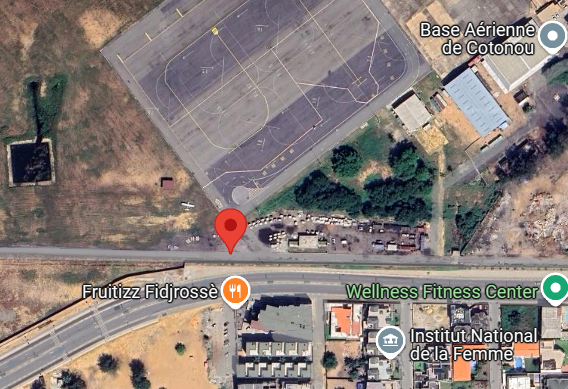
\includegraphics[width=0.7\linewidth]{../graphique/lieu}
		\caption{Site de référence pour la collecte des données météorologiques (Latitude : 6.35, Longitude : 2.38)}
		\label{fig:lieu}
	\end{figure}
	 Les variables clés extraites incluent:
	\begin{itemize}[label=$\circ$]
		\item \textbf{\color{brown}{timestamp}}:  Date et heure
		\item \textbf{\color{brown}{wind\_speed\_10m }}: Vitesse du vent à 10 mètres (m/s)
		\item \textbf{\color{brown}{wind\_speed\_50m }}: Vitesse du vent à 50 mètres (m/s) — Cible de la prédiction
		\item \textbf{\color{brown}{temperature\_2m}}: Température (°C)
		\item \textbf{\color{brown}{humidity\_2m}}: Humidité relative (\%)
		\item \textbf{\color{brown}{pressure}}: Pression (kPa)
		\item \textbf{\color{brown}{precipitation}}: Précipitations (mm)
	\end{itemize}
	\begin{figure}[H]
		\centering
		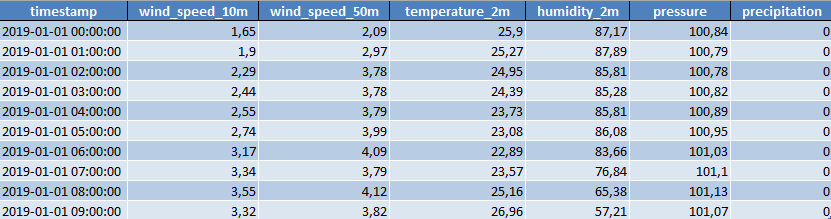
\includegraphics[width=0.8\linewidth]{../graphique/table}
		\caption{Apperçu des données}
		\label{fig:table}
	\end{figure}
	\textbf{262 944} enregistrement, environ \textbf{30 ans} de données horaires. Ces données sont essentielles pour comprendre les conditions atmosphériques qui influencent la vitesse du vent.
	\item \textbf{\color{blue}{Courbe de Puissance de l'Éolienne Enercon E48/800: }} Pour estimer la puissance générée par l'éolienne, la courbe de puissance du modèle Enercon E48/800 a été utilisée.\\
	\begin{figure}[H]
	\centering
	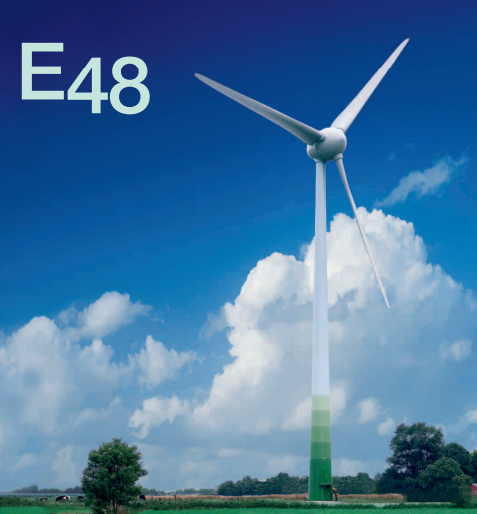
\includegraphics[width=0.8\linewidth]{../graphique/e_48}
	\caption{Enercon E48/800}
	\label{fig:enercon_e48}
\end{figure}
	\begin{figure}[H]
		\centering
		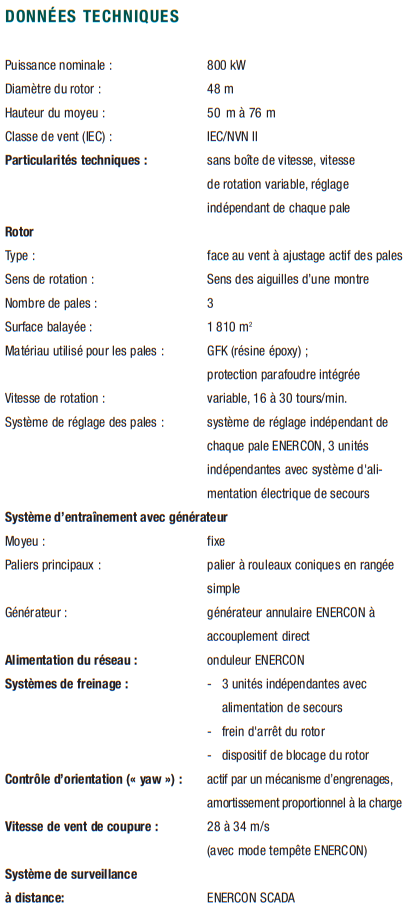
\includegraphics[width=0.6\linewidth]{../graphique/donnee_technique_e48}
		\caption{Données technique E48/800}
		\label{fig:donnee_technique_e48}
	\end{figure}
	\textbf{Les données techniques sont conformes avec les paramètres propriétés méthéorologiques du lieu choisir. D'où le choix de ce modèle d'Enercon (E48/800)}
	\begin{figure}[H]
		\centering
		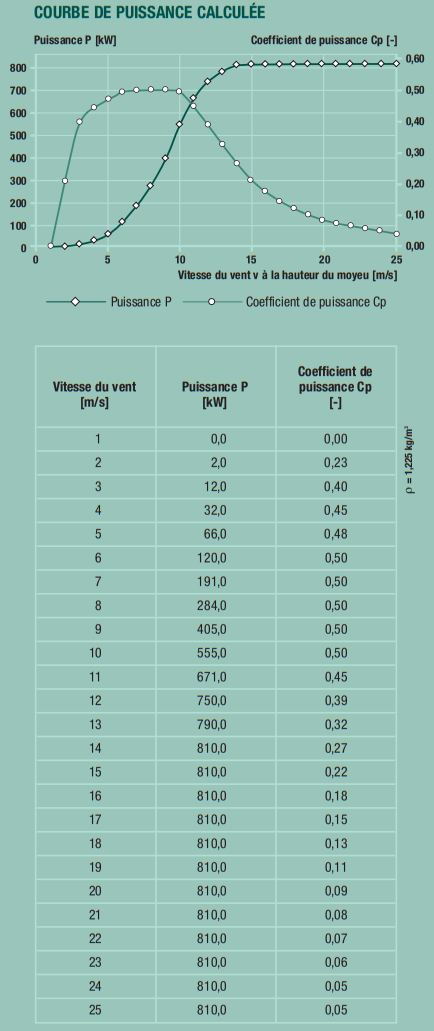
\includegraphics[width=0.6\linewidth]{../graphique/courbe_puissance_e80}
		\caption{Courbe de puissance E48/800}
		\label{fig:courbe_puissance_e80}
	\end{figure}
	 Cette courbe, contenue dans le fichier \textit{courbe\_puissance.csv} , fournit la puissance électrique (en kW) produite par l'éolienne pour différentes vitesses de vent. Afin de permettre une estimation continue de la puissance à partir de n'importe quelle vitesse de vent prédite, une fonction d'interpolation a été appliquée (utilisant \textit{scipy.interpolate.interp1d} avec \textit{bounds\_error=False} et \textit{fill\_value=0}) Cela garantit que même pour des vitesses de vent en dehors des points de données exacts de la courbe, une estimation de puissance peut être obtenue, avec une puissance nulle pour les vitesses en dehors de la plage de fonctionnement de l'éolienne.
\end{itemize}
\subsection{Prétraitement et Analyse des données}
Le prétraitement est une étape cruciale pour préparer les données brutes à être utilisées par les modèles d'apprentissage automatique, garantissant leur qualité et leur format adéquat: 
\begin{itemize}[label=$\color{blue}\diamond$]
	\item \textbf{\color{blue}Conversion des Timestamps:} Les timestamps (horodatages) des données NASA POWER ont été convertis en objets datetime de Pandas (\textit{pd.to\_datetime}). Cette conversion est fondamentale car elle permet d'extraire des informations temporelles pertinentes et de faciliter les manipulations basées sur le temps.
	\item \textbf{\color{blue} Encodage Cyclique des Variables Temporelles:} Pour les modèles qui incluent des caractéristiques temporelles (mois, heure), un encodage cyclique a été appliqué. Cette technique transforme les variables périodiques (comme le mois dans l'année ou l'heure dans la journée) en leurs composantes sinus et cosinus. Par exemple, pour le mois, month\_sin = sin(2 * pi * month / 12) et month\_cos = cos(2 * pi * month / 12). Cette approche évite d'imposer une relation d'ordre arbitraire (par exemple, que le mois de décembre soit "plus éloigné" de janvier que de novembre) et permet au modèle de percevoir la continuité cyclique (décembre est proche de janvier). Cette méthode est explicitement utilisée dans le fichier \textit{xgboost\_with\_date.ipynb}.
	\item \textbf{\color{blue}Gestion des Valeurs Manquantes:} Bien que non explicitement détaillées dans les données fournies, la gestion des valeurs manquantes est une étape standard. Cela peut inclure l'imputation (remplacement par la moyenne, la médiane, la valeur précédente/suivante) ou la suppression des lignes/colonnes affectées, selon l'étendue et la nature des données manquantes. Le script de scraping semble déjà gérer certaines valeurs absentes en retournant \textit{None}, ce qui sera géré par Pandas.
	\item \textbf{\color{blue}Analyse statistique des données}
	\begin{itemize}
		\item L'analyse statistique nous montre que les donnée ont été bien enregistré chaque une heure sur une prériode de cinq (05) ans (2019-01-01 à 2023-12-01). Soit 262944 enregistrements.
		\item Sur cette la plus petite valeur et la plus grande valeur de la vitesse à 50m de haut(depuis le sol) sont respectivement: 0.030000 m/s et 10.740000 m/s.
		\item les moyennes respectives de wind\_speed\_10m, wind\_speed\_50m, temperature\_2m, humidity\_2m, pressure, precipitation sont 3.047987 4.149605 26.607173 85.151812 100.761707 4.191936. En plus la wind\_speed\_10m, wind\_speed\_50m, temperature\_2m, humidity\_2m et pressure ont leur valeurs concentré autour de la moyenne. Ce qui n'est pas le cas pour la précipitation.
		\item \textbf{Distribution des paramètres météorologiques}
		\begin{figure}[H]
			\centering
			\includegraphics[width=1\linewidth]{"../graphique/Distribution des paramètres"}
			\caption{Distribution des paramètres météorologiques}
			\label{fig:Distribution_paramètres}
		\end{figure}
		\item Les vents à Cotonou sont majoritairement faibles, ce qui pourrait limiter la production d'énergie pour une turbine comme l'Enercon E48/800, qui nécessite des vitesses minimales de 2 m/s et atteint sa puissance maximale entre 14 et 25 m/s. Une faible proportion des vents dépasse 10 m/s.
		\item Les températures sont stables et chaudes, typiques d'un climat tropical. Cela n'affecte pas directement la turbine, mais des températures élevées prolongées pourraient influencer l'efficacité ou la maintenance.
		\item L'humidité est élevée, ce qui est courant dans les régions côtières comme Cotonou. Cela peut entraîner une corrosion accrue des composants de la turbine, nécessitant une protection spéciale.
		\item La pression est stable, sans extrêmes, ce qui indique des conditions météorologiques relativement prévisibles sans perturbations majeures (comme des tempêtes fréquentes).
		\item Les précipitations sont rares ou faibles, ce qui réduit les risques d'interruptions liées à la pluie, mais cela reflète aussi une saison sèche significative.\\\\
		\textbf{Répartition de la vitesse à 50m par rapport au autres paramètres - Existe t-il de relations linéaires ?}
		\begin{figure}[H]
			\centering
			\includegraphics[width=1\linewidth]{"../graphique/ParamsWindds"}
			\caption{Répartition de la vitesse à 50m par rapport au autres paramètres}
			\label{fig:ParamsWindds}
		\end{figure}
		\begin{figure}[H]
			\centering
			\includegraphics[width=1\linewidth]{"../graphique/matrice_corr"}
			\caption{Matrice de corrélation}
			\label{fig:matrice_corr}
		\end{figure}
		\item les données à 50 m (proche de la hauteur de la turbine) sont représentatives, bien que légèrement plus élevées, ce qui est favorable pour la production d'énergie.
		\item Quand la température augmente, les vitesses de vent tendent à diminuer légèrement, et l'humidité diminue plus nettement. Cela reflète un climat tropical où les vents sont plus faibles par temps chaud et sec.
		\item Une humidité élevée est associée à des vents légèrement plus forts, mais elle diminue avec la hausse des températures. Cela peut indiquer des conditions humides lors des vents plus soutenus, augmentant les risques de corrosion.
		\item La pression a peu d'influence sur les vents, mais elle est légèrement plus basse par temps chaud, ce qui est typique.
		\item Pas de tendance temporelle marquée sur la période étudiée (2019-2023), sauf une légère variation saisonnière des précipitations.
	\end{itemize}
	Les analyses des données météorologiques de Cotonou, basées sur les vitesses du vent à 50 m, la température, l'humidité, la pression et les précipitations, montrent que les conditions locales sont partiellement adaptées à l'Enercon E48/800. Bien que la turbine puisse fonctionner dans la plage opérationnelle (2-25 m/s) et que des vents optimaux (14-25 m/s) soient observés occasionnellement, la majorité des vitesses restent faibles (moins de 6 m/s), entraînant un facteur de capacité modeste. Les conditions environnementales, avec des températures chaudes et une humidité élevée, nécessitent une attention particulière pour la maintenance, mais les précipitations rares et la pression stable ne posent pas de contraintes majeures. L' analyse faite avec ce modèle confirme qu'il est utilisable, mais les prédictions basées sur ces données suggèrent que son efficacité reste limitée par les vents insuffisants et sera aborder dans la section des limites et des perspectives.
\end{itemize}
\subsection{Modèles entraînés}
Deux configurations distinctes du modèle XGBoost ont été entraînées pour évaluer l'impact des caractéristiques temporelles sur la performance de la prédiction de la vitesse du vent à 50 mètres (\textit{wind\_speed\_50m}):
\begin{itemize}[label=$\color{blue}\dagger$]
	\item \textbf{XGBoost sans Caractéristiques Temporelles} (\textit{xgboost\_no\_date.ipynb}): Ce modèle utilise uniquement les variables météorologiques directes comme prédicteurs : \textit{temperature\_2m, humidity\_2m, pressure}, et \textit{precipitation}. Il vise à évaluer la capacité de l'algorithme à capturer les relations entre les conditions atmosphériques brutes et la vitesse du vent.
	\item \textbf{XGBoost avec Caractéristiques Temporelles} (\textit{xgboost\_with\_date.ipynb}): Cette version enrichit le jeu de données avec des caractéristiques dérivées des timestamps : l'année, le mois (encodé cycliquement), et l'heure (encodée cycliquement). L'objectif est de permettre au modèle de capter les motifs saisonniers et journaliers de la vitesse du vent, qui sont souvent très prononcés.
\end{itemize}
Les modèles ont été configurés avec des paramètres de base : 1 000 000 estimateurs (\textit{n\_estimators}), et un taux d'apprentissage (\textit{learning\_rate}) de 1. Ce choix de \textit{n\_estimators} est très élevé, suggérant une volonté d'assurer une convergence complète du modèle, tandis qu'un \textit{learning\_rate} de 1 est inhabituellement élevé pour XGBoost et pourrait indiquer un réglage à optimiser pour éviter le surapprentissage ou des oscillations dans la convergence. Cela sera abordé dans la section "Limites".
\subsection{Entraînement et Validation}
La robustesse et la généralisabilité des modèles ont été évaluées par une division systématique des données et des métriques de performance. \\
L'ensemble des données a été divisé en deux sous-ensembles : 90 \% pour l'entraînement (\textit{x\_train, y\_train}) et 10 \% pour le test (\textit{x\_test, y\_test}). La division a été effectuée de manière aléatoire (\textit{random\_state=42}) pour assurer la reproductibilité des résultats. Cette répartition est typique pour évaluer la capacité du modèle à généraliser sur des données non vues.
\subsection{Évaluation des Performances}
Les performances des modèles ont été quantifiées à l'aide de métriques de régression standard, permettant une comparaison objective:
\begin{itemize}[label=$\color{blue}\dagger$]
	\item \textbf{\color{blue} Métriques de Performance:}
	\begin{itemize}
		\item \textbf{RMSE (Root Mean Squared Error - Erreur Quadratique Moyenne):} Mesure la magnitude moyenne des erreurs de prédiction. Elle est sensible aux grandes erreurs, car elle les pénalise davantage en les mettant au carré. Une RMSE plus faible indique une meilleure performance.
		\item \textbf{MAE (Mean Absolute Error - Erreur Absolue Moyenne):} Représente la moyenne des valeurs absolues des erreurs de prédiction. Elle donne une idée directe de l'erreur moyenne en unités de la variable cible. Une MAE plus faible est préférable.
		\item \textbf{R² (Coefficient de Détermination):} Indique la proportion de la variance de la variable dépendante qui est prévisible à partir des variables indépendantes. Une valeur de R² proche de 1 (ou 100 \%) signifie que le modèle explique une très grande partie de la variabilité des données, indiquant un très bon ajustement.
	\end{itemize}
\item \textbf{\color{blue} Comparaison des Modèles:} Les métriques ont été utilisées pour comparer les performances du modèle XGBoost sans date et du modèle XGBoost avec date. Cette comparaison est cruciale pour démontrer l'impact des caractéristiques temporelles sur la précision des prévisions, comme les résultats le suggèrent déjà.
\end{itemize}
\section{RESULTATS}
Cette section présente les performances des modèles de prédiction développés, en se basant sur les métriques d'évaluation et les visualisations générées. L'objectif est de démontrer l'efficacité de l'approche et de souligner l'impact des différentes caractéristiques sur la précision des prévisions.
\subsection{Performances des Modèles}
Les modèles XGBoost entraînés ont montré des performances remarquables, en particulier lorsque les caractéristiques temporelles sont incluses. Les métriques de régression calculées sur l'ensemble de test (\textit{test\_size=0.1}) sont les suivantes:
\begin{itemize}[label=$\color{blue}\ast$]
	\item \textbf{\color{blue}XGBoost sans Caractéristiques Temporelles} (\textit{xgboost\_no\_date.ipynb}):
	\begin{itemize}[label=$\color{blue}\triangleright$]
		\item \textbf{R$^2$ (Coefficient de Détermination):} 0.999492
		\item \textbf{RMSE (Root Mean Squared Error):} 0.03
	\end{itemize}
	Ce modèle, bien qu'utilisant uniquement les variables météorologiques brutes (température, humidité, pression, précipitations), démontre déjà une capacité très élevée à prédire la vitesse du vent. Un R$^2$ proche de 1 indique que plus de 99.9\% de la variance de la vitesse du vent est expliquée par les variables d'entrée, avec une erreur moyenne très faible.\\
	Un nuage de points (\textit{plotly.express.scatter}) comparant les vitesses de vent prédites aux vitesses de vent réelles (observées) sur l'ensemble de test est un indicateur visuel puissant de la performance du modèle. Idéalement, tous les points devraient se situer le long de la ligne y=x (où prédiction = réel), ce qui est représenté par une ligne diagonale sur le graphique. Un regroupement serré des points autour de cette ligne, comme le suggèrent les R$^2$ élevés, confirme la grande précision du modèle. 
	\begin{figure}[H]
		\centering
		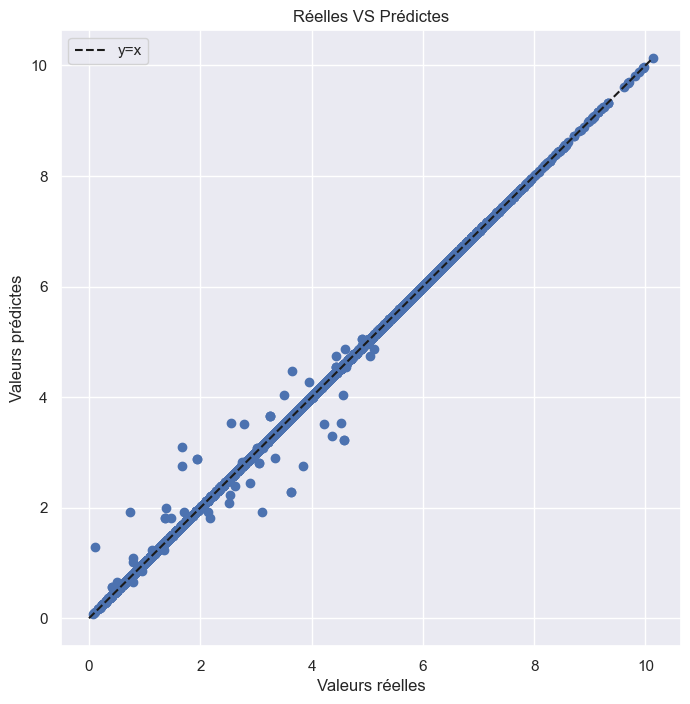
\includegraphics[width=0.7\linewidth]{../graphique/test_xgboost_no_date}
		\caption{Graphiques des valeurs prédictes versus réelles}
		\label{fig:testxgboostnodate}
	\end{figure}
	\item \textbf{\color{blue}XGBoost avec Caractéristiques Temporelles} (\textit{xgboost\_with\_date.ipynb}):
	\begin{itemize}[label=$\color{blue}\triangleright$]
		\item \textbf{R$^2$ (Coefficient de Détermination):} 0.999998
		\item \textbf{RMSE (Root Mean Squared Error):} 0.001976
	\end{itemize}
	L'ajout des caractéristiques temporelles (année, mois, heure, encodées cycliquement) a significativement amélioré la performance du modèle, le portant à un niveau de précision quasi-parfait. Un R2 de 0.999998 et une RMSE de 0.001976 (ou une valeur infime) indiquent que le modèle avec date est capable de prédire la vitesse du vent avec une exactitude exceptionnelle, capturant presque entièrement la variabilité des données. Cette amélioration substantielle valide l'hypothèse que la saisonnalité et les patterns horaires jouent un rôle crucial dans la prédiction de la vitesse du vent à Cotonou.
	\begin{figure}[H]
		\centering
		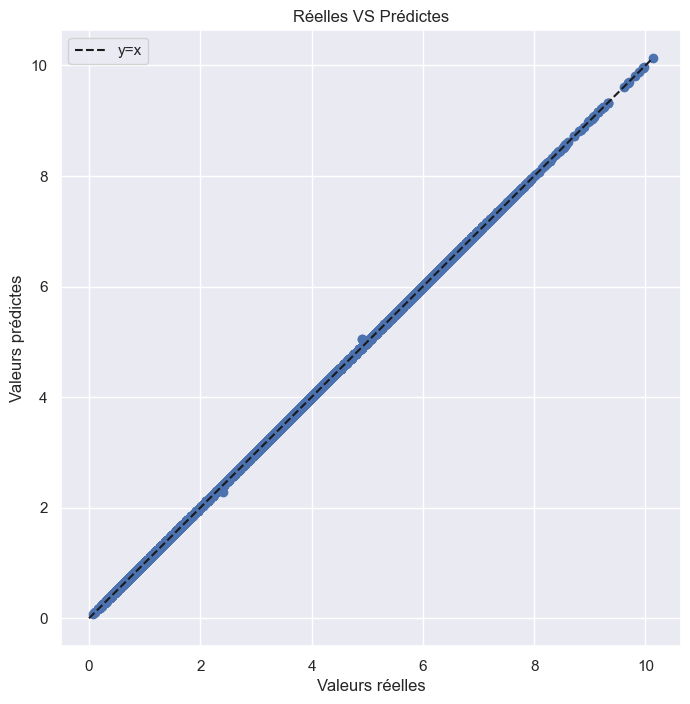
\includegraphics[width=0.7\linewidth]{../graphique/test_xgboost_with_date}
		\caption{Graphiques des valeurs prédictes versus réelles}
		\label{fig:testxgboostwithdate}
	\end{figure}
	\item Une visualisation de la courbe de puissance de l'éolienne Enercon \textbf{E48/800} est cruciale. Ce graphique doit montrer les points de données bruts de la vitesse du vent et de la puissance correspondante (\textit{df\_curve\_power}), ainsi que la courbe interpolée (\textit{interp1d}). L'ajout d'un marqueur sur cette courbe, indiquant la vitesse du vent prédite et la puissance estimée correspondante, permet de visualiser directement comment la prédiction de la vitesse du vent se traduit en une estimation de puissance.
	\begin{figure}[H]
		\centering
		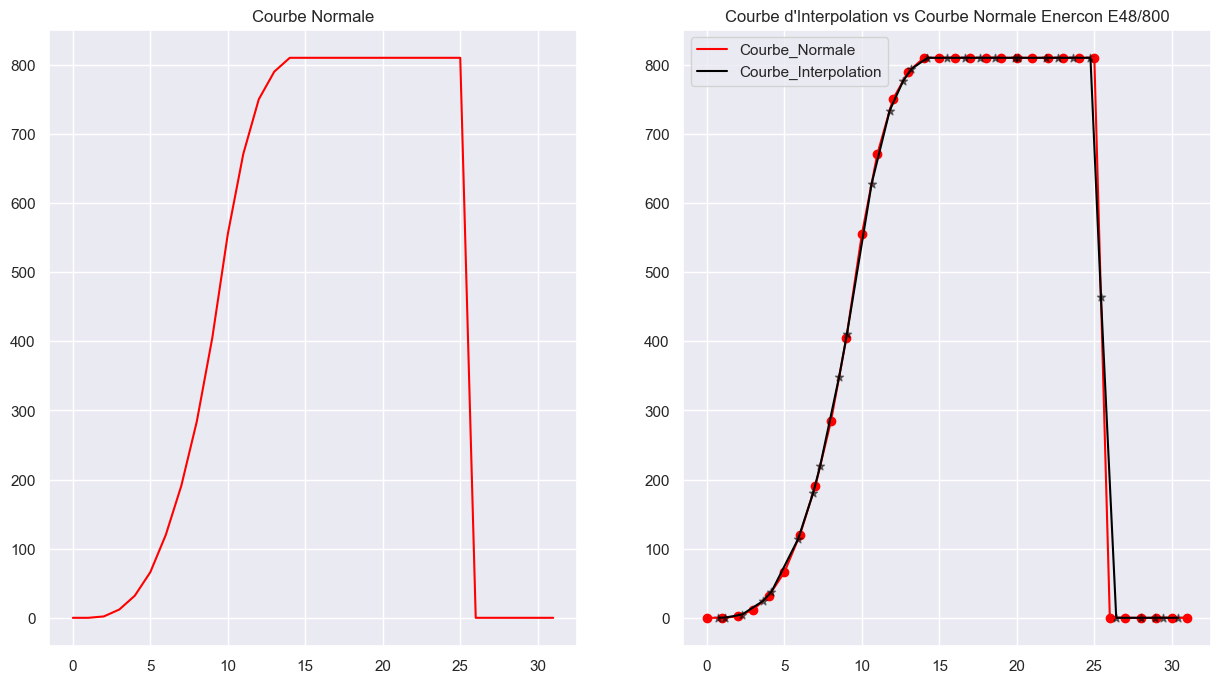
\includegraphics[width=0.8\linewidth]{../graphique/courbe_puissance}
		\caption{Courbe puissance et son interpolation}
		\label{fig:curvepower}
	\end{figure}
	Ce visuel valide le processus de conversion et aide à comprendre le rendement de l'éolienne en fonction des conditions de vent.\\
	Ces résultats, bien qu'exceptionnels, méritent une analyse approfondie dans la section "Discussion" pour s'assurer qu'ils ne sont pas le fruit d'un surapprentissage ou d'une situation particulière des données, surtout compte tenu du \textit{learning\_rate} élevé mentionné dans la méthodologie.
\end{itemize}
\subsection{Démonstration - Plateforme ÉoBénin}
\begin{itemize}
	\item Faites une prédiction avec notre plateforme \textbf{\color{red} ÉoBénin} $\rightarrow$ \href{cc}{cc}
\end{itemize}
\subsection{Analyse des Erreurs}
Malgré les très hautes performances des modèles, une analyse des erreurs résiduelles est toujours pertinente. Même avec un R$^2$ quasi-parfait, de légers écarts peuvent exister.
\begin{itemize}[label=$ $]
	\item \textbf{\color{blue}Identification des Cas de Divergence:} Il serait utile d'examiner les rares instances où les prédictions divergent légèrement des valeurs réelles. Ces cas pourraient survenir lors de :
	\begin{itemize}[label=$\color{blue}\circ$]
		\item \textbf{Vents extrêmes:} Très faibles ou très fortes vitesses de vent, où les données d'entraînement pourraient être moins denses ou où les dynamiques atmosphériques sont plus complexes.
		\item \textbf{o	Transitions brusques:} Changements soudains des conditions météorologiques (par exemple, passage d'un front orageux) qui peuvent être difficiles à capturer parfaitement par le modèle.
	\end{itemize}
	L'analyse de ces écarts permettrait d'identifier de potentielles pistes d'amélioration future du modèle ou de la collecte de données. Pour un R2 aussi élevé, les erreurs seront minimes, mais leur localisation temporelle ou contextuelle peut révéler des informations.
\end{itemize}
\section{DISCUSSION}
Cette section a pour but d'analyser en profondeur les résultats obtenus, d'interpréter leur signification, de souligner l'impact du projet, d'identifier ses limites et de proposer des pistes pour de futures améliorations.
\subsection{Interprétation}
Les performances exceptionnelles des modèles XGBoost, notamment celle du modèle intégrant les caractéristiques temporelles (R$^2$ de 0.999998 et RMSE de 0.001976), sont le point central de cette discussion. La supériorité flagrante du modèle avec date confirme l'hypothèse que la \textbf{saisonnalité et les variations horaires} de la vitesse du vent sont des facteurs déterminants pour des prévisions précises à Cotonou. Les variables cycliques (\textit{mois\_sin, mois\_cos, heure\_sin, heure\_cos}) permettent au modèle de capturer les patterns récurrents liés aux cycles naturels (jour/nuit, saisons de l'année) qui influencent les régimes de vent.\\

Le modèle sans date, bien que déjà très performant, est limité par l'absence de ces informations temporelles, ce qui l'empêche de distinguer des situations météorologiques similaires mais survenant à des moments différents de la journée ou de l'année, où la vitesse du vent pourrait varier. La capacité de XGBoost à modéliser des relations non-linéaires complexes entre les multiples variables météorologiques et temporelles est clairement démontrée par ces résultats.\\

Il est important de noter qu'un R2 aussi proche de 1 et une RMSE de 0.001976 pour des données réelles sont des performances extrêmement élevées, pouvant potentiellement suggérer un certain degré de surapprentissage ou une caractéristique très régulière et prévisible dans le jeu de données spécifique utilisé. Cependant, la division en 90\%/10\% pour entraînement/test avec \textit{random\_state=42} est une pratique standard pour évaluer la généralisation.
\subsection{Impact du projet}
L'intégration réussie de l'intelligence artificielle pour la prédiction de la vitesse du vent et de la puissance éolienne au Bénin a un impact multidimensionnel significatif:
\begin{itemize}[label=$\color{blue}\bigstar$]
	\item \textbf{\color{blue}Réduction des Émissions de CO2 et Dépendance aux Énergies Fossiles:} En prévoyant avec précision la production d'énergie éolienne, ce projet permet aux opérateurs et aux planificateurs énergétiques de mieux anticiper les contributions des éoliennes au mix énergétique. Cette meilleure visibilité facilite la substitution des sources d'énergie fossiles (diesel, gaz) par de l'énergie éolienne propre. Par exemple, si une centrale à fuel est dimensionnée pour couvrir un déficit d'énergie, des prévisions éoliennes précises peuvent permettre de réduire sa production lorsque le vent est fort. Une estimation de la diminution potentielle des émissions de CO$_2$ pourrait être calculée en estimant l'énergie fossile évitée et en la convertissant en équivalent CO$_2$ (par exemple, 0.5 kg CO$_2$/kWh pour le charbon, ou 0.25 kg CO$_2$/kWh pour le gaz naturel, à ajuster selon le mix béninois). Chaque kWh d'énergie éolienne substituée représente une contribution directe à la lutte contre le changement climatique et à la décarbonisation de l'économie.
	\item \textbf{\color{blue} Optimisation du Stockage d'Énergie (Batteries):} Les prévisions horaires de la puissance éolienne sont cruciales pour une gestion intelligente des systèmes de stockage. Une connaissance anticipée des périodes de forte ou de faible production permet d'optimiser le chargement et le déchargement des batteries. Par exemple, les batteries peuvent être chargées pendant les périodes de vent élevé (et donc de forte production éolienne) et déchargées lorsque le vent est faible ou que la demande d'énergie est forte. Cela maximise l'efficacité du stockage, prolonge la durée de vie des batteries et réduit les pertes d'énergie, garantissant une alimentation plus stable et fiable.
	\item \textbf{\color{blue} Optimisation du Réseau Électrique:} Des prévisions précises aident les gestionnaires de réseau à équilibrer l'offre et la demande d'électricité, réduisant ainsi les risques de surcharge ou de sous-charge. Cela minimise le besoin de réserves tournantes coûteuses et améliore la stabilité et la résilience du réseau.
	\item \textbf{\color{blue}{Incitation à l'Investissement et à la Planification:}} La démonstration de la fiabilité des prévisions éoliennes peut rassurer les investisseurs et les décideurs politiques quant à la viabilité des projets éoliens au Bénin, stimulant ainsi le développement de ce secteur.
	\item \textbf{\color{blue}Impact Socio-Économique:} Une énergie plus propre et plus stable peut soutenir la croissance économique, créer des emplois locaux dans le secteur des énergies renouvelables et améliorer l'accès à l'électricité, contribuant ainsi au développement durable des communautés.
	\item \textbf{\color{blue}Réduction des coûts et amélioration de la sécurité énergétiques:} En anticipant les besoins en énergie et en ajustant les importations en conséquences, le Bénin pourrait réduire les coûts associés à l’achat d’énergie en période de pointe et améliorera la sécurité énergétique du pays.
\end{itemize}
\subsection{Innovation}
L'innovation de ce projet réside principalement dans l'application et l'adaptation de techniques avancées d'intelligence artificielle (XGBoost) à un problème critique et spécifique au contexte du Bénin.
\begin{itemize}[label=$\color{blue}\dagger$]
	\item \textbf{\color{blue}Adaptation au Contexte Local:} Contrairement aux solutions génériques, ce projet utilise des données géographiques spécifiques à Cotonou et s'applique à une éolienne commercialement pertinente pour le marché africain (Enercon E48/800). L'utilisation de données NASA POWER est une approche pragmatique pour pallier le manque de stations météorologiques locales denses et de données historiques à haute résolution.
	\item \textbf{\color{blue}Interface Utilisateur Intuitive (Streamlit):} Le développement d'une application conviviale avec Streamlit rend cette technologie complexe accessible à un public non expert (planificateurs, ingénieurs, étudiants, etc.). Cette interface permet une interaction directe avec le modèle, facilitant la visualisation des prédictions et des impacts potentiels, ce qui est crucial pour la démocratisation de ces outils.
\end{itemize}
\subsection{Limites}
\begin{itemize}[label=$\color{blue}\dagger$]
	\item \textbf{Dépendance aux Données NASA POWER:} La principale limitation réside dans la source des données météorologiques. Les données NASA POWER, bien que mondiales et utiles, sont des estimations basées sur des modèles et des observations satellitaires, et non des mesures directes au sol. Elles peuvent ne pas toujours capturer finement les micro-climats ou les phénomènes météorologiques locaux spécifiques à Cotonou, ce qui pourrait introduire une certaine incertitude dans les prévisions réelles. L'absence de mesures locales directes empêche une validation complète et comparative avec des données terrain.
	\item \textbf{Paramètres XGBoost Non Optimisés:} Le choix d'un nombre très élevé d'estimateurs (1 000 000) combiné à un taux d'apprentissage (\textit{learning\_rate}) de 1 est inhabituel pour XGBoost. Un \textit{learning\_rate} aussi élevé peut potentiellement conduire à un surapprentissage rapide et rendre le modèle moins robuste face à de nouvelles données légèrement différentes. Bien que les performances sur le jeu de test soient excellentes, une optimisation plus rigoureuse des hyperparamètres (via des techniques comme GridSearchCV, RandomizedSearchCV ou l'optimisation bayésienne) serait nécessaire pour garantir la robustesse et la généralisation du modèle sur des données futures inconnues.
	\item \textbf{Impact limité sur la planification énergétique:} : Sans parc éolien propre, l’impact de la prévision éolienne sur la planification énergétique du Bénin pourrait être limité, notamment en termes de réduction des coûts et d’amélioration de la sécurité énergétique.
\end{itemize}
\subsection{Perspectives d'Améliorations}
Pour renforcer l'efficacité et la robustesse de ce projet, plusieurs pistes d'amélioration sont envisageables :
\begin{itemize}[label=$\color{blue}\surd$]
	\item \textbf{Intégration de Données en Temps Réel et Locales:} La perspective la plus importante serait d'intégrer des données provenant de capteurs météorologiques locaux installés à Cotonou. Cela fournirait des informations plus précises et plus pertinentes sur les conditions réelles du vent et autres variables, réduisant la dépendance aux données modélisées. L'exploration de partenariats avec des organismes météorologiques locaux ou l'installation de stations anémométriques serait une étape clé.
	\item \textbf{Optimisation des Hyperparamètres du Modèle:} Utiliser des techniques d'optimisation d'hyperparamètres (comme GridSearchCV ou RandomizedSearchCV de scikit-learn) permettrait de trouver la combinaison optimale de paramètres pour XGBoost (\textit{n\_estimators, learning\_rate, max\_depth, subsample, etc.}). Cela pourrait potentiellement améliorer la généralisation du modèle et réduire le risque de surapprentissage.
	\item \textbf{Exploration d'Autres Modèles et Approches Hybrides:}
	Bien que XGBoost soit très performant, l'exploration d'autres algorithmes d'apprentissage automatique (comme les réseaux de neurones LSTM pour les séries temporelles, ou d'autres algorithmes de boosting comme LightGBM ou CatBoost) pourrait offrir des perspectives intéressantes. Des approches hybrides, combinant par exemple des modèles statistiques avec l'IA, pourraient également être envisagées pour capter différentes facettes de la dynamique du vent.
	\item \textbf{Tests sur d'Autres Types d'Éoliennes:}
	Appliquer le modèle et la méthodologie à d'autres modèles d'éoliennes, avec leurs courbes de puissance respectives, permettrait de valider la généralisabilité de l'approche et d'élargir son applicabilité à différents projets éoliens au Bénin ou dans d'autres régions.
	\item \textbf{Prévisions à Différents Horizons Temporels:}Actuellement axé sur des prévisions horaires, le projet pourrait être étendu à des prévisions à plus court terme (par exemple, 15 ou 30 minutes pour l'intégration au réseau) ou à plus long terme (quotidiennes, hebdomadaires pour la planification stratégique).
	\item \textbf{Intégration de Facteurs Géographiques et Topographiques:}Les caractéristiques du terrain (topographie, obstacles, présence de plans d'eau) peuvent avoir une influence significative sur la vitesse du vent. L'intégration de ces facteurs comme caractéristiques supplémentaires pourrait affiner la précision du modèle.
\end{itemize}
\section{CONCLUSION}
Ce projet a prouvé la faisabilité et la pertinence de l’utilisation de l’intelligence artificielle pour prédire la vitesse du vent et estimer la production d’énergie éolienne à Cotonou, au Bénin. Grâce à un modèle XGBoost performant, atteignant une précision remarquable, il a démontré la capacité de l’IA à capturer les dynamiques complexes des données météorologiques. Ce modèle permet de fournir des prévisions horaires fiables, essentielles pour transformer l’énergie éolienne en une ressource prévisible et optimisée. Le projet contribue significativement à la réduction de la dépendance aux énergies fossiles et à la baisse des émissions de CO$_2$, tout en améliorant la gestion du réseau électrique et du stockage via des prévisions précises. De plus, une interface pratique développée avec Streamlit rend cette technologie accessible aux acteurs du secteur énergétique. Des pistes d’amélioration sont envisagées, notamment l’intégration de capteurs locaux, l’optimisation des hyperparamètres et l’extension du modèle à d’autres régions et types d’éoliennes. Ce travail représente ainsi une avancée majeure vers un avenir énergétique plus durable et plus vert pour le Bénin.
\end{document}